\documentclass[12pt]{exam}

\usepackage[utf8]{inputenc}  % For UTF8 source encoding.
\usepackage{amsmath}  % For displaying math equations.
\usepackage{amsfonts} % For mathematical fonts (like \mathbb{E}!).
\usepackage{upgreek}  % For upright Greek letters, such as \upvarphi.
\usepackage{wasysym}  % For additional glyphs (like \smiley!).
\usepackage{mathrsfs} % For script text (hash families and universes).
\usepackage{enumitem}
\usepackage{graphicx}
% For document margins.
\usepackage[left=.8in, right=.8in, top=1in, bottom=1in]{geometry}
\usepackage{lastpage} % For a reference to the number of pages.
\usepackage[table,xcdraw]{xcolor}
\usepackage{pdfpages}
\usepackage{verbatim}

% TODO: Enter your name here :)
\newcommand*{\authorname}{Luis A. Perez}

\newcommand*{\duedate}{Wednesday, July 17th}
\newcommand*{\duetime}{11:59 pm}

% Fancy headers and footers
\headrule
\firstpageheader{EE 263\\Summer 2019}{Homework 3 \\ }{Due: \duedate\\at \duetime}
\runningheader{EE 263}{Homework 3}{\authorname}
\footer{}{\footnotesize{Page \thepage\ of \pageref{LastPage}}}{}

% Exam questions.
\newcommand{\Q}[1]{\question{\large{\textbf{#1}}}}
\qformat{}  % Remove formatting from exam questions.

% Useful macro commands.
\newcommand*{\bigtheta}[1]{\Theta\left( #1 \right)}
\newcommand*{\bigo}[1]{O \left( #1 \right)}
\newcommand*{\bigomega}[1]{\Omega \left( #1 \right)}
\newcommand*{\prob}[1]{\text{Pr} \left[ #1 \right]}
\newcommand*{\ex}[1]{\text{E} \left[ #1 \right]}
\newcommand*{\var}[1]{\text{Var} \left[ #1 \right]}

\newcommand*{\norm}[1]{\left\lVert #1 \right\rVert}
\newcommand*{\HH}{\mathscr{H}}   % Family of hash functions.
\newcommand*{\UU}{\mathscr{U}}   % Universe.
\newcommand*{\eps}{\varepsilon}  % Epsilon.


% Custom formatting for problem parts.
\renewcommand{\thepartno}{\roman{partno}}
\renewcommand{\partlabel}{\thepartno.}

% Framed answers.
\newcommand{\answerbox}[1]{
\begin{framed}
\hspace{\fill}
\vspace{#1}
\end{framed}}

\printanswers

\setlength\answerlinelength{2in} \setlength\answerskip{0.3in}

\begin{document}
\title{EE 263 Homework 3}
\author{\authorname}
\date{}
\maketitle
\thispagestyle{headandfoot}
\setcounter{MaxMatrixCols}{15}

\begin{questions}
%%%%%%%%%%%%%%%%%%%%%%%%%%%%%%%%%%%
\Q{Fitting a model for hourly temperature}

  \begin{solution}
    \begin{enumerate}[label=(\alph*)]
      \item In order to find $a \in \mathbb{R}$ and $p \in \mathbb{R}^N$ (which is 24-periodic) that minimizes the RMS value of $y - \hat{y}$, we can rephrase our original predictor model as a linear system:
      $$
        \hat{y} = Ax
      $$
      where $\hat{y} \in \mathbb{R}^N$ and $x \in \mathbb{R}^{25}$, which represents our parameters (since $p$ is 24-periodic). More precisely, we have:
      \[
        x =
          \begin{bmatrix}
            p_{24} \\
            p_{23} \\
            \vdots \\
            p_2 \\
            p_1 \\
            a
          \end{bmatrix} \in \mathbb{R}^25
      \]
      What is the same of $A$. In fact, we have the following:
      \[
        A =
          \begin{bmatrix}
            1 & 0 & 0 & \cdots & 0 & N \\
            0 & 1 & 0 & \cdots & 0 & N - 1 \\
            0 & 0 & 1 & \cdots & 0 & N - 2 \\
            \vdots & \vdots & \vdots & \ddots & \vdots & \vdots \\
            0 & 0 & 0 & \cdots & 1 & N - 23 \\
            1 & 0 & 0 & \cdots & 0 & N - 24 \\
            0 & 1 & 0 & \cdots & 0 & N - 25 \\
            0 & 0 & 1 & \cdots & 0 & N - 26 \\
            \vdots & \vdots & \vdots & \ddots & \vdots & \vdots 
          \end{bmatrix} \in \mathbb{R}^{N \times 25}
      \]
      This means that $A$ is a skinny and tall matrix, for an over-constrained system of equations. Finding the $x$ that minimizes the RMS of $\hat{y} - y$ can be done by computing:
      \[
        x = (A^TA)^{-1}A^Ty
      \]
      The $x$ above give use $p$ as well as $a$. 

      \item We now perform the process described in part (a). The trend parameter is:
      \[
        a=-0.012075460503471858
      \]
      A plot of the predictions as well as the observed values can be seen in Figure \ref{fig:temperatures_on_train}.

      \item 
        The RMSE of the prediction error for tomorrow's temperatures is: 
        \[
          0.6521628280735887
        \]

        A plot of the predicted and observed temperatures for tomorrow can be seen in Figure \ref{fig:temperatures_on_test}.
    \end{enumerate}
  \end{solution}

  \begin{figure}[!ht]
    \centering
    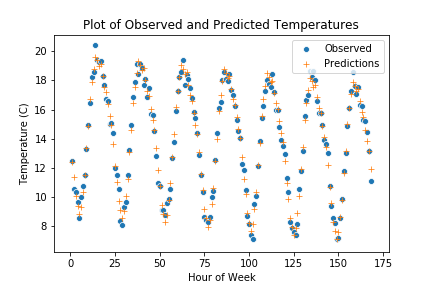
\includegraphics{figures/temps_on_train.png}
    \caption{Plot of predicted (x) and observed (o) temperatures on training data.}
    \label{fig:temperatures_on_train}
  \end{figure}
  \begin{figure}[!ht]
    \centering
    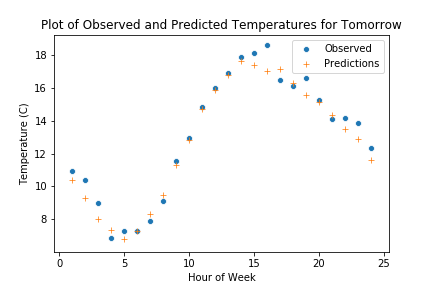
\includegraphics{figures/temps_on_test.png}
    \caption{Plot of predicted (x) and observed (o) temperatures on test data.}
    \label{fig:temperatures_on_test}
  \end{figure}

\Q{Identifying a system from input/output data}

  \begin{solution}
    \begin{enumerate}[label=(\alph*)]
      \item We wish to find $A$ such that:
       \[
        J = \sum_{k=1}^N || Ax^{(k)} - y^{(k)}||^2
       \]
       is minimized. Taking the derivative wrt. $A$, we have:
       \begin{align*}
        \frac{\partial J}{\partial A} &= \frac{\partial}{\partial A} \left[\sum_{k=1}^N || Ax^{(k)} - y^{(k)}||^2 \right ] \\
        &= \sum_{k=1}^N \frac{\partial}{\partial A}\left[ || Ax^{(k)} - y^{(k)}||^2 \right ] \\
        &= \sum_{k=1}^N \frac{\partial}{\partial A}\left[ (Ax^{(k)} - y^{(k)})^T(Ax^{(k)} - y^{(k)}) \right ] \\
        &= 2\sum_{k=1}^N  (Ax^{(k)} - y^{(k)}) x^{(k)}^T \\
        &= 2A \sum_{k=1}^N x^{(k)}x^{(k)}^T - 2\sum_{k=1}^N  y^{(k)}x^{(k)}^T
       \end{align*}
       So setting equal to $0$ and solving for $A$, we have:
       \begin{align*}
        A &= \left(\sum_{k=1}^N  y^{(k)}x^{(k)}^T\right)\left(\sum_{k=1}^N x^{(k)}x^{(k)}^T \right)^{-1}
       \end{align*}
       So we can find $A$ if and only if the second term above is invertible.

       \item Implementing the method discussed above, we obtain the following $A$:
       \[
        \hat{A} =
          \begin{bmatrix}
            2.02992454 &  5.02077879 &  5.01040266 \\
            0.0114300076 &  6.99991043 &  1.01061265 \\
            7.04239020 & 0 &  6.94476335 \\
            6.99765743 &  3.97592792 &  4.00242122 \\
            9.01295285 &  1.04493868 &  6.99800225 \\
            4.01187599 &  3.96488792 &  9.02674982 \\
            4.98710794 &  6.97233996 &  8.03363399 \\
            7.94249406 &  6.08754514 &  3.01735388 \\
            0 &  8.97218370 & -0.0385465462 \\
            1.06123427 &  8.02076138 &  7.02847693
          \end{bmatrix}
       \]
       This gives us a realtive error of $0.05814323689487761$.
    \end{enumerate}
  \end{solution}

\Q{Robust regression using the Huber penalty function}

  \begin{solution}
    \begin{enumerate}[label=(\alph*)]
      \item We our parameter vector be $w = \begin{bmatrix} w_1 \\ 2_2 \end{bmatrix}$.
    \end{enumerate}
  \end{solution}

\Q{Identifying a system from input/output data}

  \begin{solution}
    \begin{enumerate}[label=(\alph*)]
      \item TODO
    \end{enumerate}
  \end{solution}

\end{questions}

\begin{comment}
\includepdf[
    %% Include all pages of the PDF
    pages=-,
    %% make this page have the usual page style
    %% (you can change it to plain etc). By default pdfpages
    %% sets the pagecommand to \pagestyle{empty}
    pagecommand={\pagestyle{headings}}]
%% The pdf file itself
{HW3Code.pdf}
\end{comment}















\end{document}
